% !TEX program = pdflatex
\documentclass[conference]{IEEEtran}

\usepackage[utf8]{inputenc}
\usepackage[T1]{fontenc}
\usepackage{amsmath,amssymb}
\usepackage{booktabs}
\usepackage{array}
\usepackage{tabularx}
\usepackage{multirow}
\usepackage{graphicx}
\usepackage{xcolor}
\usepackage{url}
\usepackage[hidelinks,unicode]{hyperref}
\usepackage{enumitem}
\usepackage{float}
\usepackage{balance}

\graphicspath{{figures/}}

\renewcommand{\arraystretch}{1.15}
\setlist[itemize]{leftmargin=*,topsep=2pt,itemsep=1pt,parsep=0pt}
\setlist[enumerate]{leftmargin=*,topsep=2pt,itemsep=1pt,parsep=0pt}

\newcommand{\risk}{\textit{at-risk}}
\newcommand{\oulad}{OULAD}
\newcommand{\grain}{\texttt{id\_student + code\_module + code\_presentation}}
\newcommand{\metric}[1]{\textbf{#1}}
\newcolumntype{Y}{>{\raggedright\arraybackslash}X}
\newcolumntype{R}{>{\raggedleft\arraybackslash}p{1.55cm}}
\newcolumntype{L}[1]{>{\raggedright\arraybackslash}p{#1}}
\newcolumntype{C}[1]{>{\centering\arraybackslash}p{#1}}

\title{
Learning Behavior Analytics and Personalized Learning Path Recommendation on Online Learning Platforms\\
\vspace{0.5cm}
\large A Focused Study on At-Risk Learners
\thanks{Final report for the DDM -- Data-Driven Marketing course. The report is prepared in a conference-paper structure, following the course template and the empirical results in the project repository.}
}

\author{
\IEEEauthorblockN{Group 7: Ha Quang Minh, Bui Huynh Gia Huy, Ngo Hoang Phuc, Nguyen Tran Quoc Dat, Truong Duc Anh}
\IEEEauthorblockA{
DSEB 65B\\
Course: DDM -- Data-Driven Marketing
}
}

\begin{document}
\maketitle

\begin{abstract}
This report presents a system for learning behavior analytics and personalized learning path recommendation on an online learning platform, while also developing an early-identification branch for learners at risk of dropping out. The study uses the Open University Learning Analytics Dataset (OULAD) at the learner - module - presentation unit of analysis, covering 32,593 enrollments and 28,785 unique learners. The risk label is defined by the final outcomes \texttt{Fail} or \texttt{Withdrawn}, with an overall \risk{} rate of 52.8\%. The analytical workflow combines data cleaning and integration, exploratory data analysis, multi-horizon feature engineering, learner-profile clustering, behavior-gap-based recommendation, multi-horizon early-warning modeling, ablation testing, calibration, bootstrap confidence intervals, subgroup diagnostics, threshold cost-benefit analysis, and a ready-to-launch A/B testing design. The results show that a useful warning signal already appears at day 7, while the strongest final model is XGBoost at day 30 with threshold 0.25, achieving recall 0.9367, F2-score 0.8540, ROC-AUC 0.8467, and PR-AUC 0.8766 on the independent test set. The final system does not only predict risk; it also converts model outputs into risk bands, learner segments, recommendation paths, and intervention logic that are implemented in a Power BI dashboard to support learner-retention decisions in a Data-Driven Marketing context.
\end{abstract}

\begin{IEEEkeywords}
Learning Analytics, Personalized Recommendation, At-Risk Learners, Early Warning System, XGBoost, Power BI, A/B Testing, Data-Driven Marketing.
\end{IEEEkeywords}

%--------------------------------------------------
\section{Introduction}

The development of online education has changed how educational institutions collect and use learner data. Each learning-resource visit, click count, assignment submission time, score, registration history, and final outcome leaves a digital trace that can be used to understand learning behavior. From a Data-Driven Marketing perspective, learners on an online learning platform can be viewed as a customer group that needs to be retained, activated at the right time, and served with messages or learning paths that match their current state. Therefore, dropout is not only an educational problem but also a retention and engagement problem.

A practical challenge for online learning platforms is that learners are heterogeneous. Some learners interact consistently, submit assessments on time, and achieve high scores. Others start slowly, study irregularly, submit few assignments, or withdraw before completing the module. If a platform applies the same learning path and the same reminder mechanism to every learner, support resources will be allocated inefficiently. A stronger approach is to combine learning analytics with prediction and recommendation models to answer three managerial questions: who is at risk, when does the risk appear, and what recommendation or intervention should be provided.

This project is designed around the following logical chain:

\begin{center}
\fbox{\parbox{0.92\linewidth}{\centering
\textbf{Behavior analytics} $\rightarrow$ \textbf{Segmentation} $\rightarrow$ \textbf{Recommendation} $\rightarrow$ \textbf{Multi-horizon early warning} $\rightarrow$ \textbf{Risk bands} $\rightarrow$ \textbf{Power BI decision support} $\rightarrow$ \textbf{A/B testing readiness}
}}
\end{center}

The important distinction of this project is that it does not stop at a static classification model. The final pipeline turns behavioral data into a decision system: it describes behavior, segments learner profiles, recommends learning paths, predicts risk at days 7, 14, 21, and 30, checks model reliability, analyzes subgroup fairness, optimizes thresholds according to advising capacity, and prepares an A/B test design to validate the impact of intervention.

%--------------------------------------------------
\section{Objectives and Research Questions}

\subsection{General Objective}

The general objective is to build an online-education data analytics framework that can: (i) explain learning behavior; (ii) segment learners; (iii) generate personalized learning path recommendations; (iv) identify learners at risk of dropping out early; and (v) visualize outputs in Power BI to support targeted intervention.

\subsection{Specific Objectives}

Part I focuses on all learners. Its objectives are to analyze interaction patterns, evaluate behavioral differences by final outcome, build learner segments, and propose recommendation paths based on behavioral profiles.

Part II focuses on the \risk{} group. Its objectives are to define the risk label, build a multi-horizon feature store, compare Logistic Regression, Random Forest, and XGBoost, select thresholds under a high-recall objective, convert predicted probabilities into risk bands, analyze major risk signals, and design an early-intervention mechanism.

\subsection{Research Questions}

The report addresses the following main questions:

\begin{enumerate}
    \item What prominent learning behavior patterns exist on the online learning platform?
    \item How do early interaction, assessment scores, learning consistency, and submission discipline differ between successful learners and at-risk learners?
    \item Can learners be segmented into interpretable learning profiles that are useful for recommendation?
    \item Can the \risk{} group be identified at days 7, 14, 21, and 30 with sensitivity high enough for early intervention?
    \item Which model, feature group, and prediction horizon produce the best predictive quality?
    \item How should predictive outputs be converted into risk bands, watchlists, and learning paths to support marketing-retention decisions?
    \item How should an A/B test be designed to verify whether personalized intervention truly improves retention?
\end{enumerate}

%--------------------------------------------------
\section{Data and Research Scope}

\subsection{The OULAD Dataset}

The study uses the Open University Learning Analytics Dataset (OULAD), a public online-learning dataset containing course information, learner profiles, registration and withdrawal records, assessment metadata, scores, and interaction logs with a virtual learning environment. OULAD is suitable for this topic because it contains the three important data groups needed for the study: demographic and learning-background variables, system interaction behavior, and final learning outcomes.

\subsection{Unit of Analysis}

The unit of analysis throughout the pipeline is an enrollment of a learner in a module during a presentation, denoted as \grain{}. This grain has three advantages. First, it matches the way OULAD records learning outcomes. Second, a learner may appear in multiple modules or presentations, so enrollment-level analysis preserves contextual information. Third, this grain aligns with real intervention decisions: the platform must know which learner, in which module, and at which point in time needs support.

\subsection{Data Tables Used}

{\raggedright
The project uses seven core OULAD tables, grouped by analytical role:
\begin{itemize}
\item Learner profile and final outcome: \texttt{studentInfo}.
\item Registration and withdrawal timing: \texttt{studentRegistration}.
\item Assessment design and scores: \texttt{assessments} and \texttt{studentAssessment}.
\item Learning-resource metadata: \texttt{courses} and \texttt{vle}.
\item Daily clickstream behavior: \texttt{studentVle}.
\end{itemize}
\par}

Table~\ref{tab:final-result} summarizes the final learning outcomes that define the analytical problem and the later \risk{} target.

\begin{table}[H]
\centering
\footnotesize
\caption{Final outcome distribution in the analytical sample}
\label{tab:final-result}
\begin{tabular}{lrr}
\toprule
Final outcome & Enrollments & Analytical implication \\
\midrule
\texttt{Pass} & 12,361 & Passed the module \\
\texttt{Withdrawn} & 10,156 & Withdrew from the module \\
\texttt{Fail} & 7,052 & Did not pass \\
\texttt{Distinction} & 3,024 & Passed with distinction \\
\midrule
Total & 32,593 & 28,785 unique learners \\
\bottomrule
\end{tabular}
\end{table}

The target variable for the \risk{} branch is defined as follows:

\begin{equation}
 y_i =
 \begin{cases}
 1, & \text{if } final\_result_i \in \{Fail, Withdrawn\} \\
 0, & \text{if } final\_result_i \in \{Pass, Distinction\}
 \end{cases}
\end{equation}

Under this definition, the overall \risk{} rate is 52.8\%. This is a large proportion, showing that non-completion risk is not an exceptional event but a substantial operational problem.

\begin{figure}[t]
\centering
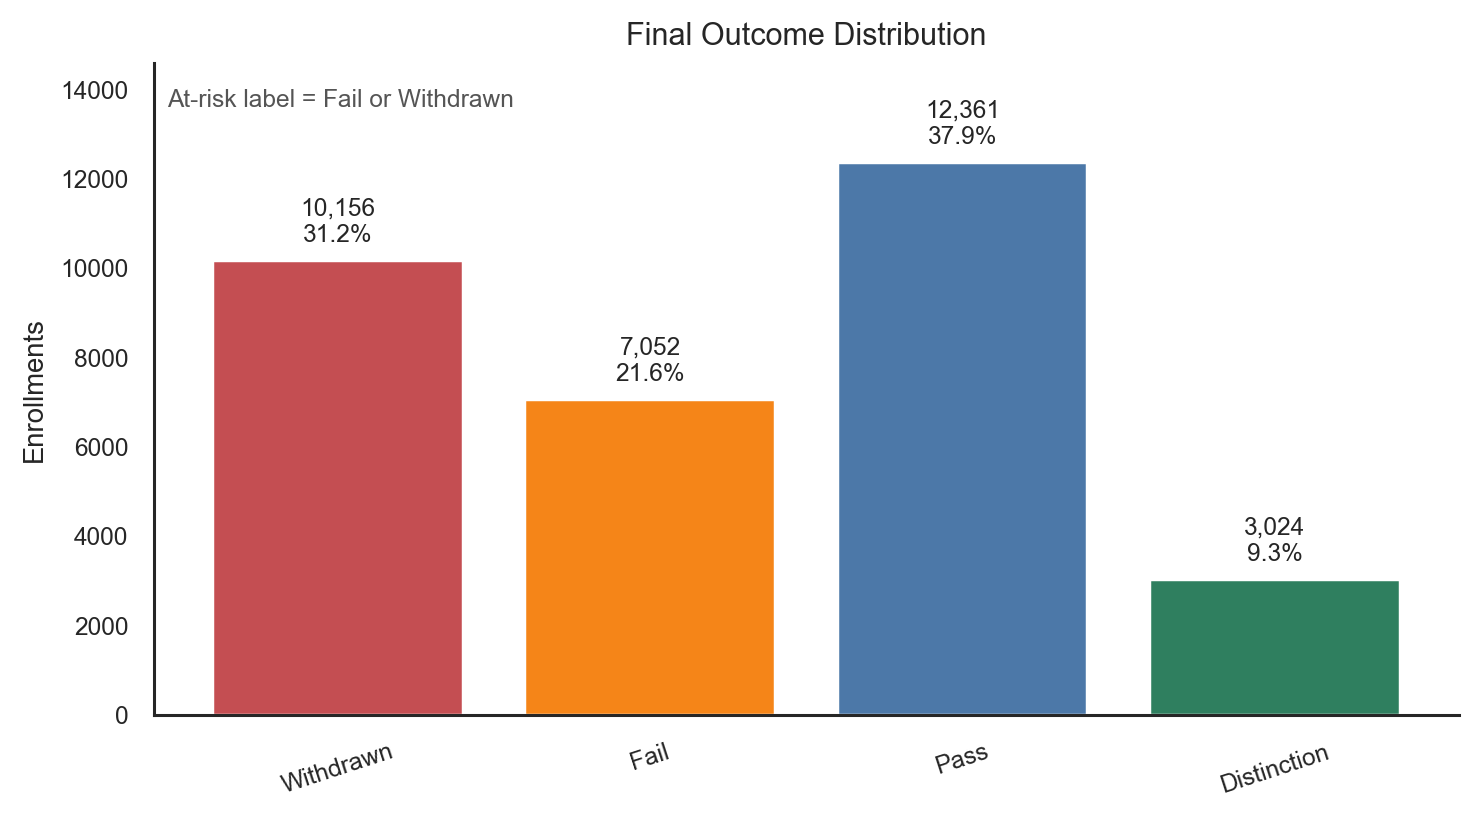
\includegraphics[width=\linewidth]{fig01_outcome_distribution.png}
\caption{Final outcome distribution and the operational at-risk definition.}
\label{fig:outcome-distribution}
\end{figure}

%--------------------------------------------------
\section{Data Preprocessing and Integration}

\subsection{Initial Data Quality Audit}

The first step is to audit each table for size, missing values, duplicates, and temporal logic. The main findings are summarized in Table~\ref{tab:cleaning}. The most notable issue is that the clickstream table \texttt{studentVle} is very large, with more than 10.6 million raw rows; therefore, aggregation by event key is required to avoid duplicated interactions.

\begin{table*}[t]
\centering
\footnotesize
\caption{Summary of raw data and main cleaning operations}
\label{tab:cleaning}
\begin{tabularx}{\textwidth}{L{3.0cm}R R Y}
\toprule
Table & Raw rows & Columns & Main checks and cleaning operations \\
\midrule
\texttt{courses} & 22 & 3 & No missing values or duplicates; used as the course and presentation-length description table. \\
\texttt{studentInfo} & 32,593 & 12 & No duplicates; \texttt{imd\_band} has 1,111 missing values, equal to 3.41\%, and is retained/standardized for subgroup analysis. \\
\texttt{studentRegistration} & 32,593 & 5 & \texttt{date\_registration} has 45 missing values and is filled using the module-presentation median; \texttt{date\_unregistration} has 22,521 missing values because many learners did not withdraw; after registration-date imputation, 21 invalid date relationships are fixed by setting the withdrawal date to missing. \\
\texttt{vle} & 6,364 & 6 & \texttt{week\_from} and \texttt{week\_to} each have 5,243 missing values; they are filled with 0 to standardize the learning-resource catalog; 20 activity types are observed. \\
\texttt{studentVle} & 10,655,280 & 6 & No missing values; 787,170 duplicated raw rows; 3,810,465 rows with the same student-site-day key are aggregated by summing \texttt{sum\_click}, producing 8,459,320 cleaned event rows; click outliers are audited using the IQR method but retained in aggregation because they may reflect real study intensity. \\
\texttt{assessments} & 206 & 6 & 11 missing deadline values; deadline and weight metadata are used for assessment features. \\
\texttt{studentAssessment} & 173,912 & 5 & 173 missing scores, equal to about 0.10\%; banked records are removed when constructing submission features to avoid signals that do not correspond to current-presentation learning behavior. \\
\bottomrule
\end{tabularx}
\end{table*}

\subsection{Integration by Enrollment Key}

After cleaning, the data are integrated by three keys: \texttt{id\_student}, \texttt{code\_module}, and \texttt{code\_presentation}. The integration principle is to keep the enrollment table at the center, then attach aggregated features from clickstream behavior, assessment behavior, and learner profiles. This ensures that all modeling, segmentation, recommendation, and Power BI tables share the same grain, avoiding over-counting caused by joining directly to detailed log tables.

\subsection{Leakage Control}

In an early-warning problem, data leakage is a major risk. A day-7 model must not use clicks, submissions, or scores occurring after day 7. Therefore, the project builds a separate feature store for each horizon: day 7, day 14, day 21, and day 30. Each table uses only the information observed up to its corresponding horizon. This design makes the horizon comparison meaningful: later horizons have richer information but leave less time for intervention.

%--------------------------------------------------
\section{Exploratory Data Analysis}

\subsection{Risk Is Unevenly Distributed Across Modules}

EDA shows that risk differs substantially across modules. The module with the highest \risk{} rate is \texttt{CCC}, at about 62.2\%, whereas the module with the lowest rate is \texttt{AAA}, at about 29.0\%. This has a direct managerial implication: the platform should not allocate support resources uniformly across all modules. Modules with a higher risk burden should be prioritized for early warnings, learning-resource redesign, or instructor support.

\subsection{Early Interaction Is a Strong Signal}

A very important insight is that risky behavior appears very early. In the first 14 days, median clicks by final outcome are:

\begin{itemize}
    \item \texttt{Distinction}: 156 clicks;
    \item \texttt{Pass}: 104 clicks;
    \item \texttt{Fail}: 40 clicks;
    \item \texttt{Withdrawn}: 12 clicks.
\end{itemize}

Figure~\ref{fig:early-behavior} visualizes the same pattern and adds the assessment-score gap. Successful outcomes have both stronger early interaction and stronger early assessment evidence, while withdrawn learners show the weakest signal on both dimensions.

\begin{figure}[t]
\centering
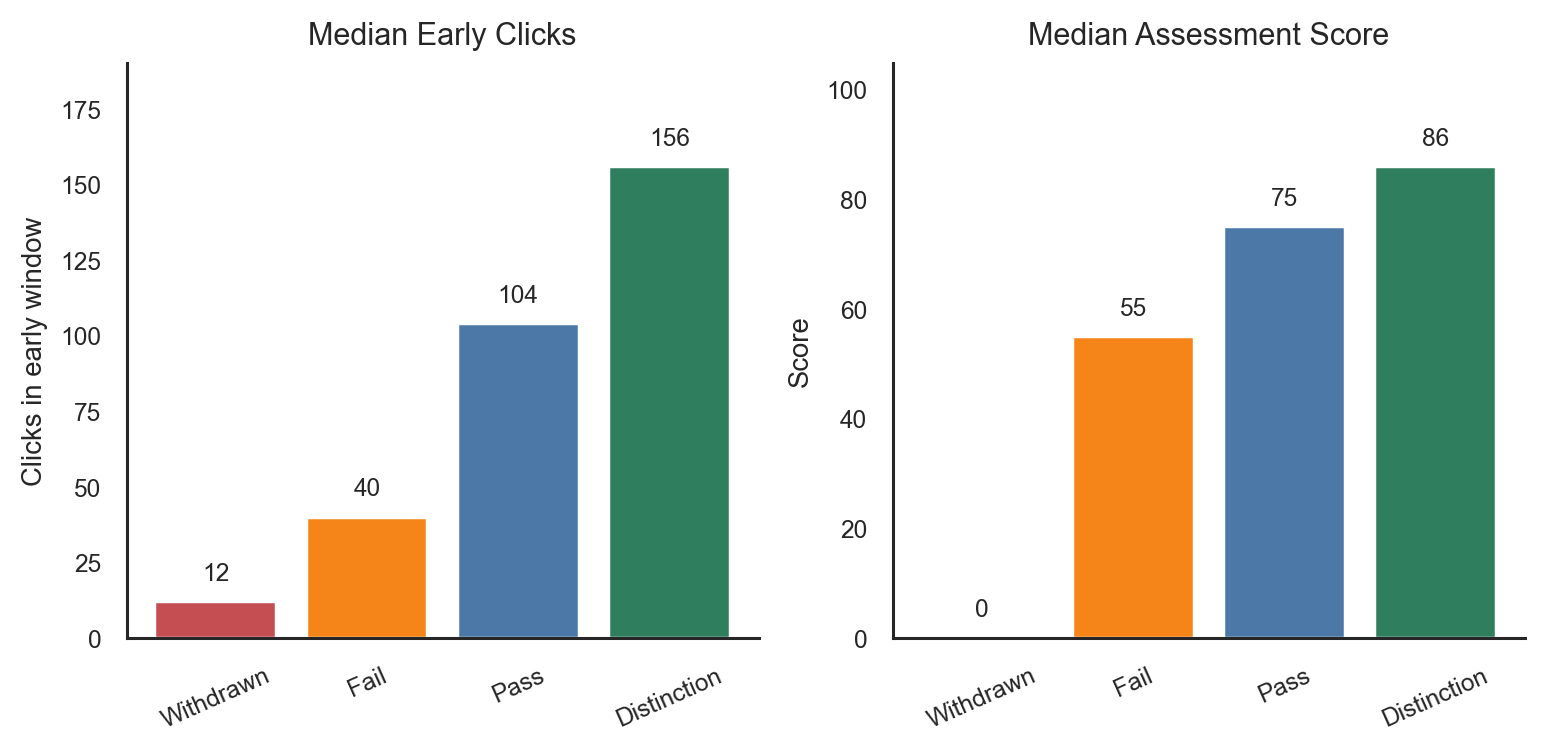
\includegraphics[width=\linewidth]{fig02_early_behavior_by_outcome.png}
\caption{Median early behavior by final outcome.}
\label{fig:early-behavior}
\end{figure}

This gap shows that learners who eventually withdraw are already far behind successful learners within the first two weeks. Therefore, the problem should be modeled as an early-warning system rather than only an end-of-course diagnostic. In marketing terms, day 7 and day 14 correspond to early retention-campaign activation checkpoints.

\subsection{Engagement Must Be Interpreted Together With Assessment}

A high number of clicks does not automatically imply a good outcome. A learner may click frequently but fail to submit assessments, or may interact less often but still pass due to strong prior ability. Therefore, EDA does not only examine \texttt{sum\_click}; it also combines active days, days since last activity, completion ratio, submission delay, and assessment scores. The core conclusion is that engagement, assessment discipline, and score quality must be included together in the feature store so that the model receives a more comprehensive signal.

%--------------------------------------------------
\section{Multi-Horizon Feature Engineering}

\subsection{Behavioral Feature Groups}

Feature engineering is organized around three signal groups: engagement, assessment, and learner profile. The main engagement variables include total clicks, active days, first and last activity dates, days since last activity, early engagement, and engagement intensity. To reduce right-skewness in click distributions, variables such as \texttt{total\_clicks}, \texttt{active\_days}, \texttt{early\_engagement}, and \texttt{engagement\_intensity} are transformed using \(\log(1+x)\).

Assessment variables include the number of submitted assessments, completion ratio, weighted average score, score standard deviation, submission delay, and an indicator for whether the learner has submitted by the horizon. Profile variables include gender, highest education, region, age band, IMD band, disability, number of previous attempts, and studied credits. Categorical variables are one-hot encoded for classification models.

\subsection{Composite Indicators}

Several composite features are designed to interpret learning behavior at a higher level:

\begin{align}
EarlyRatio_i &= \frac{EarlyEngagement_i}{TotalClicks_i}, \\
Intensity_i &= \frac{TotalClicks_i}{ActiveDays_i}, \\
Completion_i &= \frac{Submitted_i}{TotalAssessments_i}, \\
Discipline_i &= 0.5 \times Completion_i + 0.5 \times DelayNorm_i, \\
Persistence_i &= \frac{ActiveDays_i}{ActivitySpan_i}.
\end{align}

Here, \(DelayNorm\) is a normalized variable derived from submission timing; a higher value reflects better discipline. The learning risk index is constructed as:

\begin{equation}
\begin{split}
LRI_i = &0.25(1-EngNorm_i) + 0.30(1-ScoreNorm_i) \\
&+ 0.20(1-Persistence_i) + 0.15(1-Discipline_i) \\
&+ 0.10(1-EarlyNorm_i).
\end{split}
\label{eq:lri}
\end{equation}

Equation~\eqref{eq:lri} deliberately gives higher weight to score and engagement because they are the most direct signals of learning progress. However, the index also retains persistence, assessment discipline, and early engagement to reflect consistency and early study behavior.

\subsection{Coverage by Horizon}

The four prediction tables at days 7, 14, 21, and 30 each contain 32,593 rows and 40 columns, with no missing cells after imputation and no duplicate enrollment keys. Table~\ref{tab:horizon-coverage} shows the central trade-off of the project: earlier horizons leave more time for intervention but observe less assessment evidence.

\begin{table}[H]
\centering
\footnotesize
\caption{Feature-store coverage by horizon}
\label{tab:horizon-coverage}
\begin{tabular}{lrrr}
\toprule
Horizon & Activity & Submission & Score \\
\midrule
Day 7 & 74.0\% & 2.7\% & 2.7\% \\
Day 14 & 81.5\% & 10.3\% & 10.3\% \\
Day 21 & 84.7\% & 46.7\% & 46.7\% \\
Day 30 & 85.8\% & 63.8\% & 63.7\% \\
\bottomrule
\end{tabular}
\end{table}

Day 7 already has relatively high activity coverage but almost no assessment evidence. By days 21 and 30, score coverage increases sharply, helping the model rank risk more accurately. Therefore, the project does not choose a single horizon from the beginning; it evaluates the entire information curve over time.

%--------------------------------------------------
\section{Part I: Learner Segmentation and General Recommendation}

\subsection{Purpose of Segmentation}

Segmentation acts as the interpretability layer of the system. A prediction model can return a risk probability, but instructors and program managers need to understand which type of behavior a learner exhibits in order to intervene appropriately. The project uses K-Means on standardized features and combines it with rule-based interpretation to label clusters according to learning logic.

The main clustering features include total clicks, active days, early engagement, assessment score, engagement intensity, assessment discipline, persistence score, and completion ratio. All features are standardized using StandardScaler so that clusters are not dominated by the scale of click variables.

\subsection{Four Learner Segments}

The segmentation results produce four interpretable learning groups. Table~\ref{tab:segments} reports the size and \risk{} rate of each group.

\begin{table}[H]
\centering
\footnotesize
\caption{Summary of learner segments}
\label{tab:segments}
\begin{tabular}{lrrr}
\toprule
Segment & Enrollments & Share & At-risk \\
\midrule
Steady Progressors & 17,047 & 52.3\% & 39.43\% \\
Sporadic Explorers & 8,476 & 26.0\% & 60.82\% \\
Inactive Drop-offs & 5,018 & 15.4\% & 93.08\% \\
Focused Achievers & 2,052 & 6.3\% & 32.16\% \\
\bottomrule
\end{tabular}
\end{table}

\begin{figure}[t]
\centering
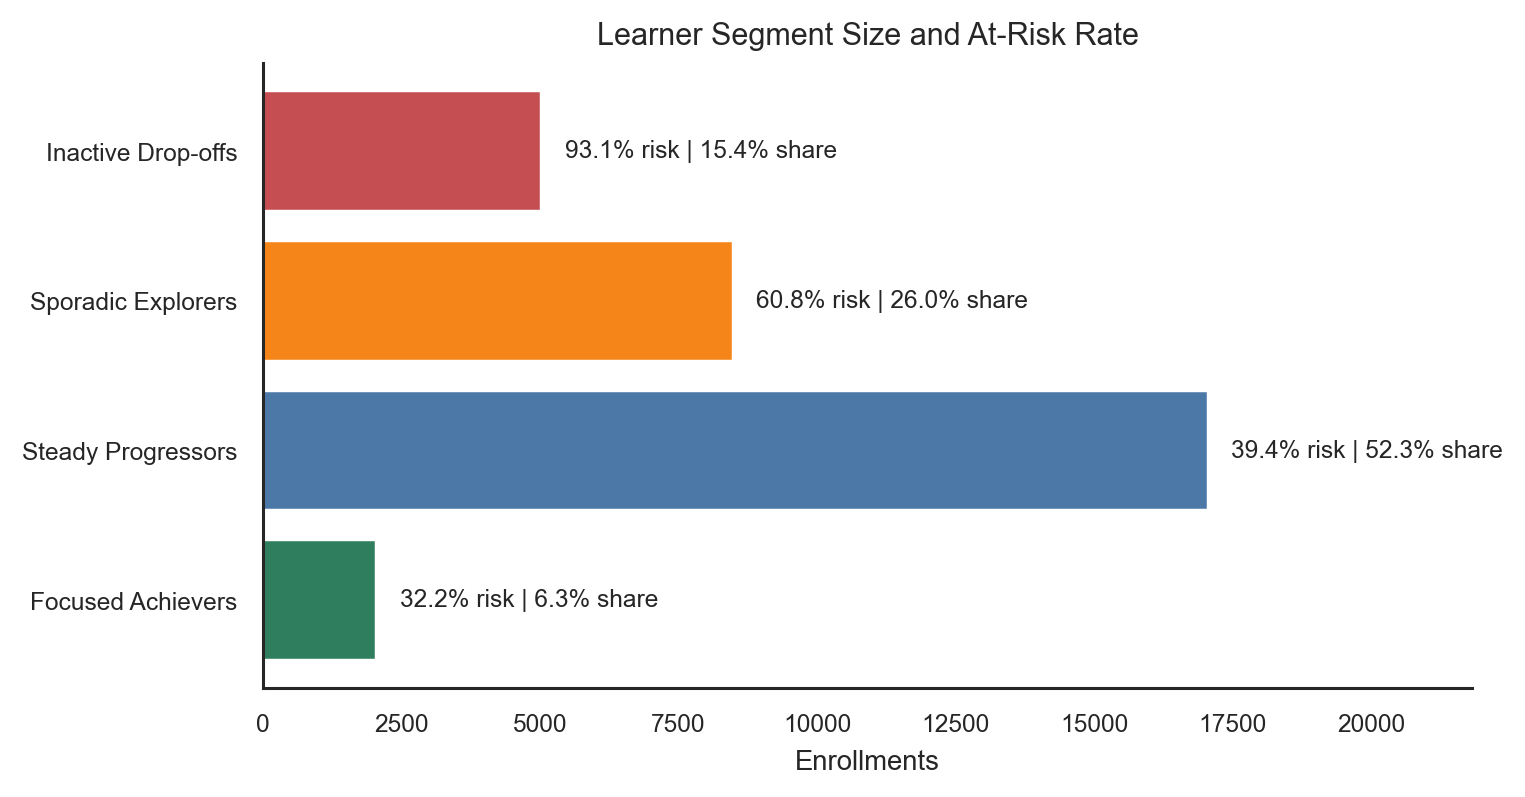
\includegraphics[width=\linewidth]{fig03_segment_risk_profile.png}
\caption{Learner segment size and at-risk rate.}
\label{fig:segment-risk-profile}
\end{figure}

\textit{Steady Progressors} is the largest segment, with relatively consistent interaction and a risk rate lower than the overall level. \textit{Sporadic Explorers} exhibit unstable behavior and need support for learning rhythm and consistency. \textit{Inactive Drop-offs} is a very high-risk segment with an \risk{} rate above 93\%, making it suitable for priority intervention. \textit{Focused Achievers} is smaller but performs better, usually requiring motivation-maintenance or advanced recommendations rather than strong risk intervention.

\subsection{Behavior-Gap-Based Recommendation}

The recommendation layer is designed to be explainable rather than algorithmically complex. The core idea is to compare the current behavior of each learner with the successful-peer profile in the same or a nearby segment, then identify which behavioral gaps should be improved. In scoring terms, a path \(p\) for learner \(i\) can be represented as:

\begin{equation}
RecScore_{i,p} = w_1 A_{p} + w_2 S_{i,p} + w_3 E_{i,p} + w_4 C_{i,p},
\end{equation}

where \(A_p\) is path accessibility, \(S_{i,p}\) is fit with similar profiles, \(E_{i,p}\) is fit with the learner's current engagement intensity, and \(C_{i,p}\) is the expected completion probability or completion-support component. In the implemented dashboard, the weights are fixed as \(w_1=0.20\), \(w_2=0.30\), \(w_3=0.25\), and \(w_4=0.25\), so the operational score is:

\begin{equation}
RecScore_i = 100 \times (0.20A_i + 0.30S_i + 0.25E_i + 0.25C_i).
\end{equation}

The highest weight is given to similar-profile fit because recommendations should be anchored in successful-peer behavior from the same segment. Engagement fit and completion support receive equal weight because the system should consider both current learning behavior and likely ability to complete. Accessibility receives a smaller but still meaningful weight, ensuring that recommended actions are practical and connected to available learning resources. This formula is used as an interpretive framework for the dashboard; Table~\ref{tab:paths} summarizes the four most common recommendation paths in the output.

\begin{table}[H]
\centering
\footnotesize
\caption{Most common recommendation paths}
\label{tab:paths}
\begin{tabular}{lr}
\toprule
Recommendation path & Enrollments \\
\midrule
Consistency Building Path & 11,133 \\
Early Start Path & 7,108 \\
Assessment Recovery Path & 5,613 \\
Mastery Improvement Path & 5,145 \\
\bottomrule
\end{tabular}
\end{table}

\textit{Consistency Building Path} fits learners with irregular interaction: the objective is to increase active days, establish a fixed study schedule, and reduce the gaps between learning sessions. \textit{Early Start Path} is for slow starters: the system should push onboarding, introductory resources, and early checkpoints. \textit{Assessment Recovery Path} is for learners with submission or low-score problems: it recommends review, practice tasks, and deadline reminders. \textit{Mastery Improvement Path} is for learners who interact reasonably well but do not score highly: it focuses on learning resources that improve understanding, reviewing assessment feedback, and practicing weak topics.

%--------------------------------------------------
\section{Part II: Identifying At-Risk Learners}

\subsection{Modeling Problem}

The prediction problem is formulated as binary classification:

\begin{equation}
P(y_i=1 \mid X_{i,h}), \quad h \in \{7,14,21,30\},
\end{equation}

where \(X_{i,h}\) is the feature vector of enrollment \(i\) observed up to horizon \(h\). The project compares three model families: Logistic Regression, Random Forest, and XGBoost. Logistic Regression is an interpretable linear baseline; Random Forest handles nonlinearities and feature interactions; XGBoost is usually strong on tabular data, especially when behavioral features and dummy variables are available.

The data are split into train, validation, and test sets in a 60\% - 20\% - 20\% ratio, stratified by the \risk{} label. The validation set is used to select thresholds and operating points; the test set is used only for final performance reporting.

\subsection{Why the 0.50 Threshold Is Not Used}

In an early-warning system, missing an at-risk learner is usually more costly than issuing an extra alert. Therefore, the default threshold of 0.50 is not appropriate. The project selects thresholds on the validation set using the following rule:

\begin{enumerate}
    \item Keep thresholds with recall \(\geq 0.90\);
    \item Among them, choose the threshold with the highest precision;
    \item If there is a tie, prioritize F2-score and then PR-AUC.
\end{enumerate}

F2-score is used because it places higher weight on recall:

\begin{equation}
F_{2} = \frac{(1+2^2) \cdot Precision \cdot Recall}{2^2 \cdot Precision + Recall}.
\end{equation}

This rule matches the early-intervention objective: capture as many at-risk learners as possible while still controlling precision so that academic advisors are not overloaded. After each model receives its own operating threshold, the horizon-level summary ranks candidate model-threshold pairs primarily by recall, then PR-AUC, F2-score, and precision. This makes the summary consistent with the purpose of the system: identify the earliest high-sensitivity warning checkpoint before optimizing for ranking quality.

\subsection{Multi-Horizon Comparison}

Table~\ref{tab:horizon-best} presents the recall-prioritized selected model at each horizon on the validation set. The results show that day 7 already provides a useful signal: Logistic Regression achieves recall 0.9393, precision 0.5771, and PR-AUC 0.7592. From day 14 onward, XGBoost becomes the stronger option, and PR-AUC increases steadily to 0.8639 at day 30.

\begin{table*}[t]
\centering
\footnotesize
\caption{Recall-prioritized selected model by horizon on the validation split}
\label{tab:horizon-best}
\begin{tabular}{l l r r r r}
\toprule
Horizon & Selected pair & Threshold & Recall & Precision & PR-AUC \\
\midrule
Day 7 & Logistic Regression & 0.25 & 0.9393 & 0.5771 & 0.7592 \\
Day 14 & XGBoost & 0.25 & 0.9372 & 0.5794 & 0.8012 \\
Day 21 & XGBoost & 0.25 & 0.9311 & 0.6122 & 0.8432 \\
Day 30 & XGBoost & 0.25 & 0.9253 & 0.6278 & 0.8639 \\
\bottomrule
\end{tabular}
\end{table*}

The key interpretation is that ranking quality improves over time, while recall remains high at all horizons. Day 7 is the earliest checkpoint that is usable for triage, whereas day 30 is the strongest checkpoint for priority ranking because it has much richer assessment evidence.

\begin{figure}[t]
\centering
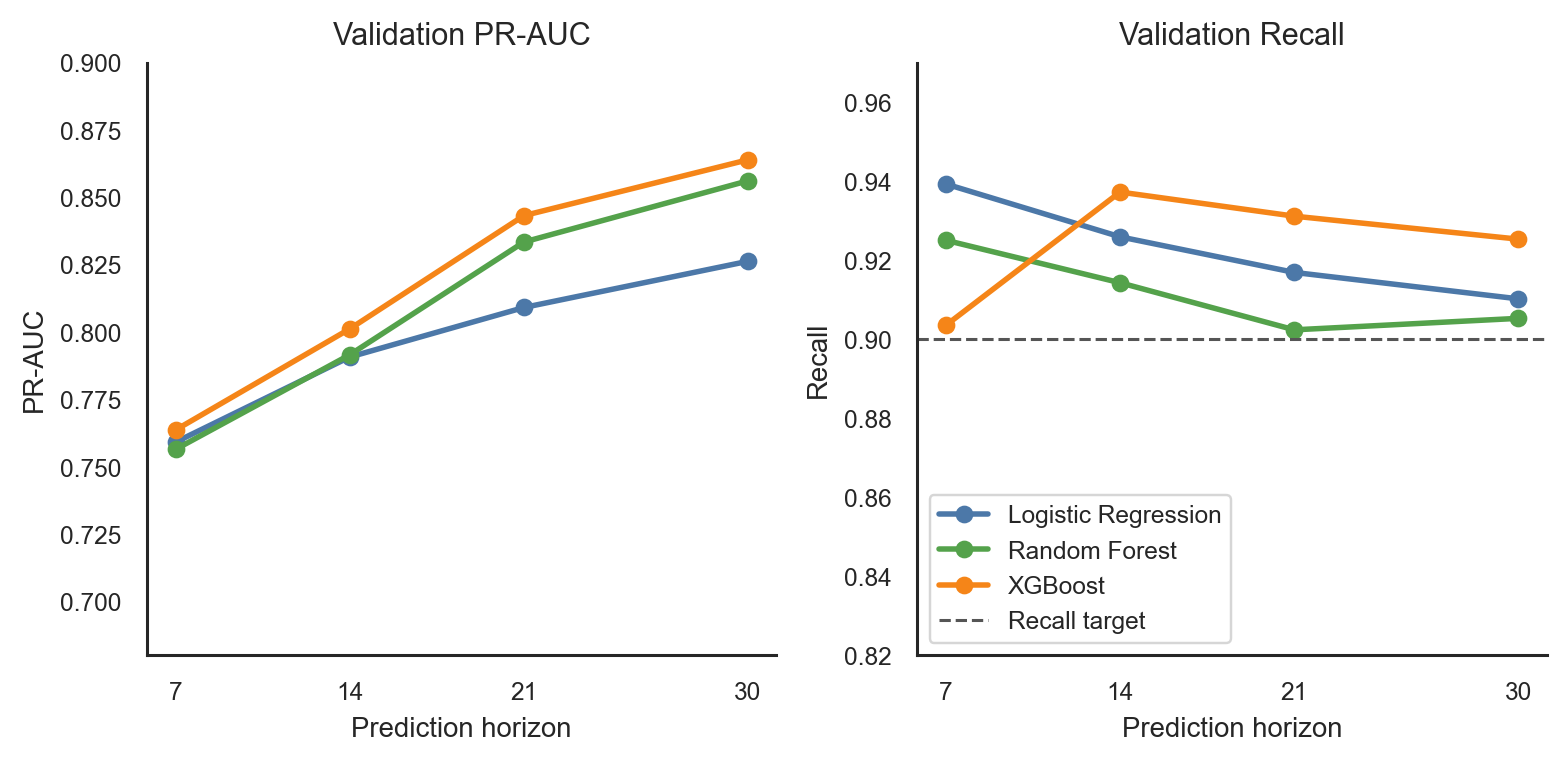
\includegraphics[width=\linewidth]{fig04_horizon_model_quality.png}
\caption{Validation PR-AUC and recall across model families and prediction horizons.}
\label{fig:horizon-quality}
\end{figure}

\subsection{Champion Model}

The final champion is XGBoost at day 30 with threshold 0.25. The model is selected based on validation performance after applying recall-oriented thresholding, then evaluated on the independent test set. Table~\ref{tab:champion} reports test performance.

\begin{table}[H]
\centering
\footnotesize
\caption{Champion model performance on the held-out test set}
\label{tab:champion}
\begin{tabular}{lr}
\toprule
Metric & Value \\
\midrule
Accuracy & 0.6777 \\
Precision & 0.6313 \\
Recall & 0.9367 \\
F1-score & 0.7542 \\
F2-score & 0.8540 \\
ROC-AUC & 0.8467 \\
PR-AUC & 0.8766 \\
Brier score & 0.1580 \\
\bottomrule
\end{tabular}
\end{table}

Recall 0.9367 means the model captures more than 93\% of at-risk enrollments in the test set. Precision 0.6313 means that about 63\% of the alerts are truly \risk{}. This is a reasonable trade-off in early intervention: the system accepts some false positives in order to reduce the chance of missing learners who need support.

%--------------------------------------------------
\section{Ablation, Calibration, and Reliability Diagnostics}

\subsection{Ablation by Feature Group}

Ablation is added to answer the question: does model performance come mainly from demographics, engagement, assessment, or a combination of signals? Table~\ref{tab:ablation} shows that the full feature set is strongest at both day 14 and day 30. In particular, demographics only reaches PR-AUC 0.6666, substantially below engagement + assessment and the full feature set.

\begin{table}[H]
\centering
\footnotesize
\caption{Ablation results by test PR-AUC}
\label{tab:ablation}
\begin{tabular}{lrr}
\toprule
Feature group & Day 14 & Day 30 \\
\midrule
Full feature set & 0.8114 & 0.8766 \\
Engagement + assessment & 0.7689 & 0.8472 \\
Engagement only & 0.7583 & 0.8033 \\
Assessment only & 0.5561 & 0.7431 \\
Demographics only & 0.6666 & 0.6666 \\
\bottomrule
\end{tabular}
\end{table}

This result has two implications. Methodologically, the model is not driven only by demographics or background characteristics; most predictive value comes from changeable behavior. Managerially, if the platform wants to reduce risk, interventions should target engagement, assessment completion, and submission discipline rather than rigidly classifying learners by personal characteristics.

\subsection{Calibration and Risk Bands}

Predicted probabilities are useful only if they are ordered and calibrated well enough to support intervention prioritization. Therefore, the project converts champion-model probabilities into four risk bands: Low, Medium, High, and Critical. Table~\ref{tab:risk-bands} shows that realized at-risk rates increase monotonically by risk band, from 15.4\% in Low to 92.5\% in Critical.

\begin{table}[H]
\centering
\footnotesize
\caption{Risk bands on the held-out test set}
\label{tab:risk-bands}
\begin{tabular}{lrrr}
\toprule
Risk band & Learners & Actual risk & Avg prob. \\
\midrule
Low & 1,412 & 15.4\% & 0.159 \\
Medium & 1,971 & 35.3\% & 0.366 \\
High & 1,232 & 62.2\% & 0.622 \\
Critical & 1,904 & 92.5\% & 0.922 \\
\bottomrule
\end{tabular}
\end{table}

Risk bands are a more operationally useful output than a single 0/1 label. In practice, academic advisors can process Critical learners first, then High, then Medium depending on available capacity. Low does not require costly intervention and can instead receive automatic nudges or self-service resources.

\begin{figure}[t]
\centering
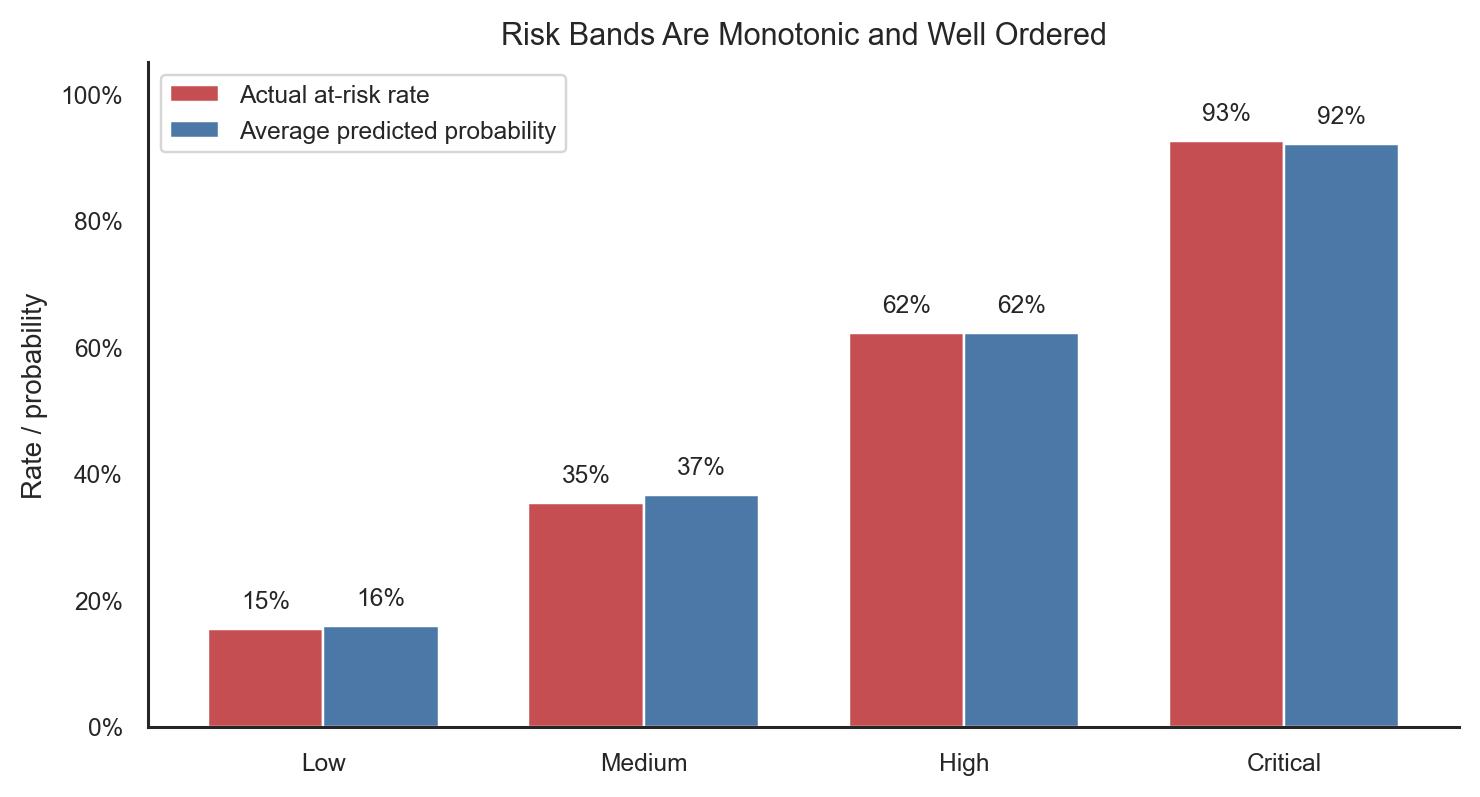
\includegraphics[width=\linewidth]{fig05_risk_band_calibration.png}
\caption{Actual at-risk rate and average predicted probability by risk band.}
\label{fig:risk-band-calibration}
\end{figure}

\subsection{Most Important Signals}

The variables with the highest global importance in the champion model include \texttt{avg\_score}, \texttt{studied\_credits}, \texttt{days\_since\_last}, \texttt{avg\_submission\_delay}, and \texttt{assessment\_discipline}. This confirms that the model is not learning only from clicks. Risk is formed by a combination of academic quality, recency of interaction, submission discipline, and study load.

\begin{figure}[t]
\centering
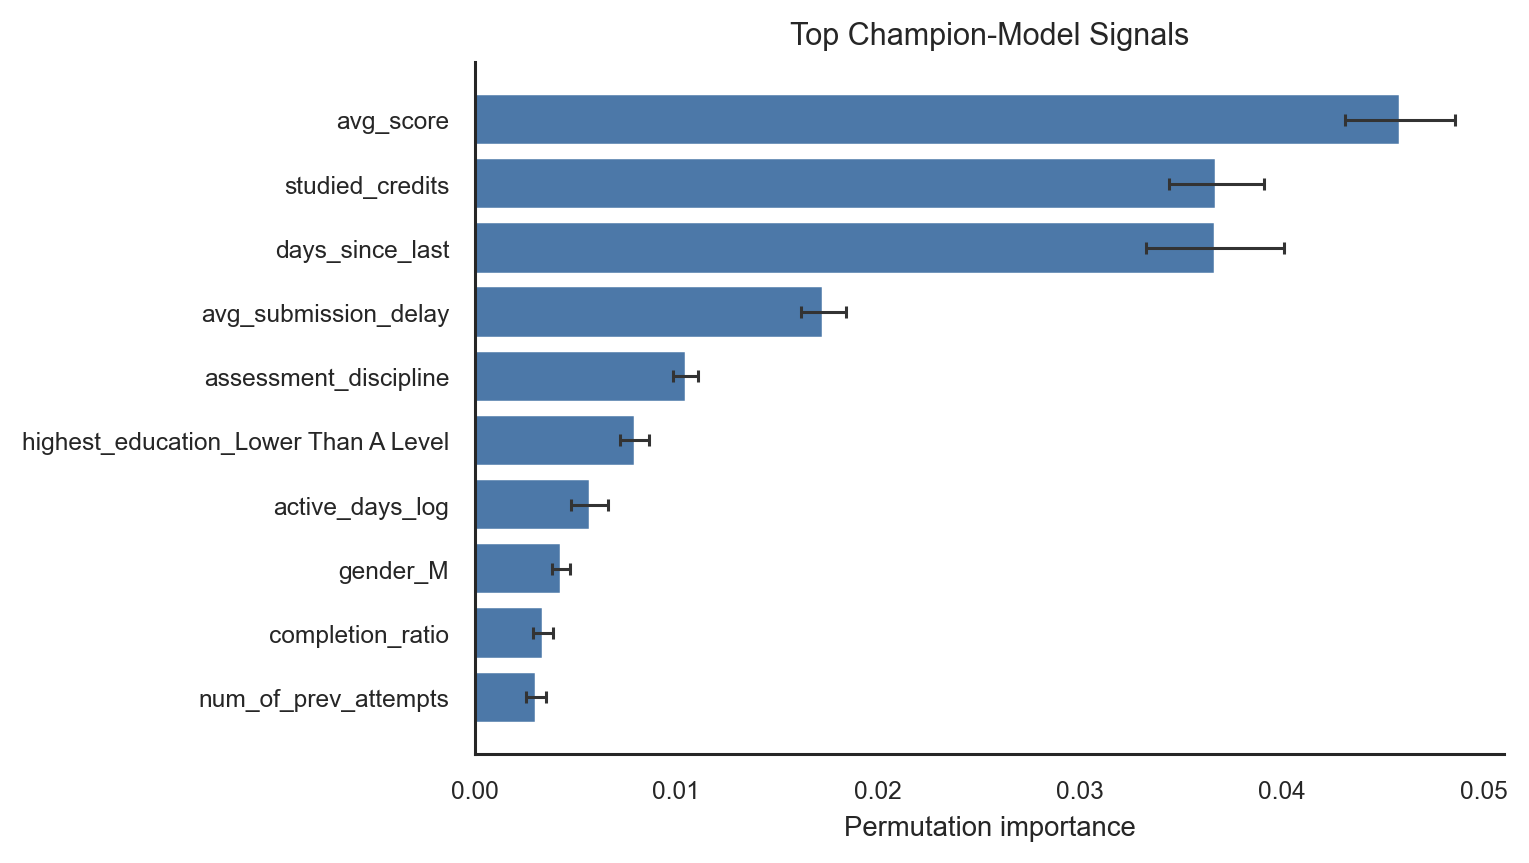
\includegraphics[width=\linewidth]{fig06_feature_importance.png}
\caption{Top champion-model signals by permutation importance.}
\label{fig:feature-importance}
\end{figure}

\subsection{Bootstrap Confidence Intervals}

To avoid relying on a single point estimate, the project bootstraps test-set metrics. Table~\ref{tab:bootstrap} shows that the 95\% confidence intervals are fairly narrow, especially for recall and PR-AUC.

\begin{table}[H]
\centering
\footnotesize
\caption{Bootstrap 95\% confidence intervals for the champion model}
\label{tab:bootstrap}
\begin{tabular}{lrrr}
\toprule
Metric & Point & CI lower & CI upper \\
\midrule
Precision & 0.6313 & 0.6173 & 0.6442 \\
Recall & 0.9367 & 0.9281 & 0.9447 \\
F1 & 0.7542 & 0.7435 & 0.7648 \\
ROC-AUC & 0.8467 & 0.8369 & 0.8559 \\
PR-AUC & 0.8766 & 0.8673 & 0.8865 \\
\bottomrule
\end{tabular}
\end{table}

The recall confidence interval from 0.9281 to 0.9447 supports the conclusion that the model is stable on the main early-warning objective. The PR-AUC interval from 0.8673 to 0.8865 also indicates consistent ranking quality.

\subsection{Subgroup Diagnostics}

The project checks performance by gender, disability, IMD band, and prior attempts. Recall remains above the 0.90 target in the checked groups. However, the high-IMD group is closest to the recall floor, at about 0.9040; the re-attempt group has lower ROC-AUC, at about 0.7625. Therefore, if the system is deployed in practice, the dashboard should monitor these groups to avoid unequal support quality.

\subsection{Segment-Level Model Performance}

At the segment level, the model performs strongest for clearly vulnerable groups: \textit{Inactive Drop-offs} has an actual at-risk rate of 93.0\% and recall 1.0000; \textit{Sporadic Explorers} has an at-risk rate of 61.6\% and recall 0.9778. For \textit{Steady Progressors}, recall is 0.8827; for \textit{Focused Achievers}, recall is 0.7163. This is reasonable because high-functioning groups have less obvious behavior: some learners have good scores but still withdraw, or interact less but still pass.

%--------------------------------------------------
\section{Warning Threshold and Intervention-Capacity Trade-Off}

Threshold 0.25 of the champion model is selected to preserve high recall. On the validation cohort, this threshold flags about 77.8\% of enrollments, catches about 488.6 \risk{} learners per 1,000 enrollments, and has a false-alert ratio of about 0.59 false positives per true positive.

In Data-Driven Marketing terms, the model creates a targeting list for a retention campaign. However, the list size is an operational-capacity decision. If academic advisors are limited, the threshold should be higher to reduce review load; if the priority is to avoid missing at-risk learners, a lower threshold is reasonable. Therefore, the dashboard should report not only precision and recall but also the number of flagged learners, the false-alert rate, and expected review load per 1,000 enrollments.

\begin{figure}[t]
\centering
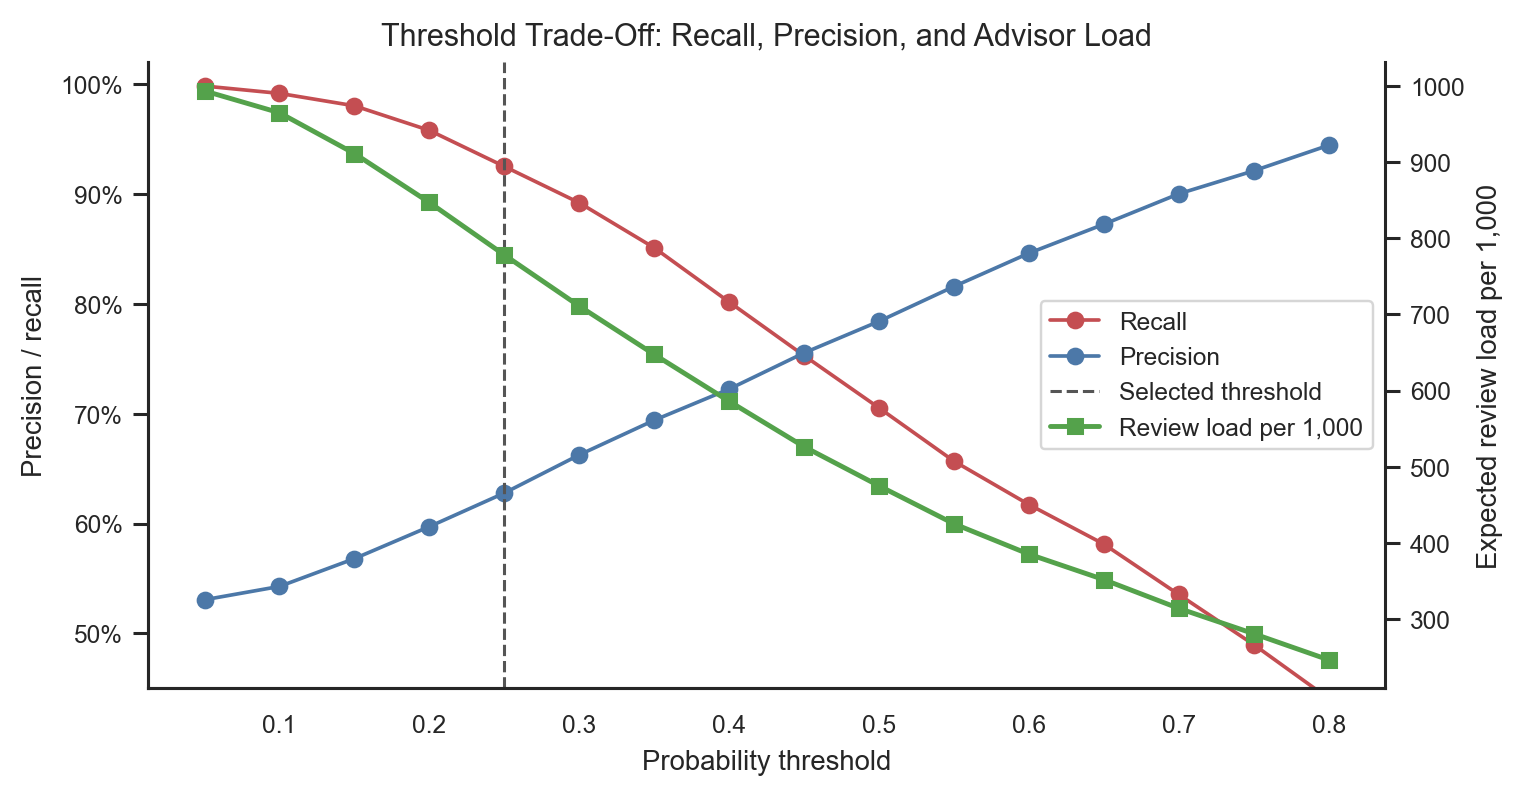
\includegraphics[width=\linewidth]{fig07_threshold_capacity_tradeoff.png}
\caption{Threshold trade-off between recall, precision, and expected advisor review load.}
\label{fig:threshold-tradeoff}
\end{figure}

%--------------------------------------------------
\section{Power BI Dashboard and Data Storytelling}

\subsection{Design Principles}

The Power BI dashboard is designed as a decision-support system, not a set of disconnected charts. The story should move from overview to action: problem scale, behavioral evidence, segmentation, recommendation, early warning, risk bands, watchlist, reliability, capacity trade-off, and A/B testing readiness.

\subsection{Final Dashboard Structure}

The submitted Power BI file is included as \texttt{powerbi/final\_share.pbix}. To align with the course outline, the dashboard is organized around six core decision pages and two advanced defense pages. The PBIX also contains supporting drill-down and definition pages for navigation, threshold review, learner-level inspection, and metric explanation. Table~\ref{tab:dashboard} describes the report logic used for presentation.

\begin{table*}[t]
\centering
\footnotesize
\caption{Final Power BI dashboard structure}
\label{tab:dashboard}
\begin{tabularx}{\textwidth}{L{3.2cm}L{3.4cm}Y}
\toprule
Page & Objective & Main KPIs / visuals \\
\midrule
Executive Overview & Present the scale and severity of the retention problem & Total enrollments 32,593; unique learners 28,785; at-risk rate 52.8\%; final outcome distribution; segment distribution; top paths; champion recall and PR-AUC. \\
Behavior \& Outcome Analytics & Show that early warning is behaviorally justified & Median early engagement, average score, completion ratio, days since last activity; module x risk heatmap; comparison of clicks/score/completion by outcome. \\
Segmentation \& Recommendation & Connect learner profiles with personalized actions & Cluster size, cluster risk rate, cluster profile heatmap, recommended path distribution, learner-level recommendation table. \\
Multi-Horizon Early Warning & Compare warning quality from day 7 to day 30 & Validation recall, precision, F2, PR-AUC by horizon-model pair; earliest useful horizon = Day 7; champion = XGBoost @ Day 30. \\
Calibration \& Model Diagnostics & Check probabilities, risk bands, and sources of predictive lift & Risk band summary, calibration chart, ablation comparison, feature importance, Brier score. \\
At-Risk Watchlist & Turn the model into a prioritized intervention list & Learner watchlist with risk probability, risk band, cluster label, recommended path, action 1/2/3; cluster x risk band matrix. \\
Reliability \& Campaign Capacity & Advanced page for model defense & Bootstrap CI, subgroup performance, risk trajectory, threshold cost-benefit, review load per 1,000. \\
A/B Experiment Readiness & Close the loop from prediction to causal validation & Eligible learners, control/treatment counts, SRM p-value, balance diagnostics, power/MDE, simulated lift scenarios. \\
\bottomrule
\end{tabularx}
\end{table*}

\subsection{Role of Power BI in the Project}

Power BI is not used only to decorate the results; it is the decision-support layer. Slicers such as module, presentation, segment, final outcome, risk band, and recommended path allow instructors or managers to move from the aggregate level to the learner-level watchlist. In a Data-Driven Marketing context, the dashboard functions as a campaign cockpit: who should be contacted, how urgent the case is, which message or learning path is appropriate, and whether the targeting threshold exceeds operational capacity. The embedded model has been checked against the exported CSV outputs, so the dashboard is ready for demonstration; refreshing it on another machine may require repointing the Power Query source folder to the repository's \texttt{data/processed} directory.

%--------------------------------------------------
\section{A/B Testing Design and Intervention Validation}

\subsection{Why A/B Testing Is Needed}

The prediction model answers the question of who is at risk, but it does not prove that personalized intervention will make learners stay or pass the module. To make a causal claim, the platform needs a randomized experiment with control and treatment groups. Therefore, the project adds an A/B testing design as the bridge from offline prediction to causal validation.

\subsection{Experiment Design}

The experiment ID is summarized as \textit{Risk Targeted Intervention A/B Test}. The randomization unit is student-course enrollment. The control group receives standard support, while the treatment group receives personalized intervention based on risk band, segment, and recommended path. The primary metric is \texttt{retention\_success}, meaning that the final outcome after intervention does not belong to the \risk{} group. Secondary metrics include recommendation score, risk probability, risk-band mix, and path uptake. Guardrails include advisor review load, false-alert ratio, and subgroup recall monitoring. Table~\ref{tab:ab} summarizes the experiment-readiness checks exported for the proposed intervention test.

\begin{table}[H]
\centering
\footnotesize
\caption{A/B testing readiness}
\label{tab:ab}
\begin{tabular}{lr}
\toprule
Indicator & Value \\
\midrule
Eligible flagged learners & 5,107 \\
Control group & 2,554 \\
Treatment group & 2,553 \\
SRM p-value & 0.9888 \\
Historical baseline success & 0.3687 \\
Minimum detectable effect & 3.82\% \\
\bottomrule
\end{tabular}
\end{table}

The SRM p-value of 0.9888 indicates no sample-ratio mismatch in the planned 50/50 allocation. With the current sample size, the offline sample is not strong enough to reliably detect an absolute lift of 3\% at 80\% power, but it is sufficient for lift scenarios of 5\%, 8\%, and 10\%. The simulated +5\% scenario has p-value 0.00026, a 95\% confidence interval from +2.32\% to +7.66\%, and satisfies the business decision rule.

\subsection{Decision Rule}

The proposed rollout rule is: deploy system-wide only if \(p < 0.05\), the 95\% confidence interval of lift excludes 0, and the lift is large enough to matter operationally. This rule helps avoid two common mistakes: relying only on p-values while ignoring business significance, or seeing a large lift in a simulation/historical split and deploying without causal evidence.

%--------------------------------------------------
\section{Managerial Implications and Learning Path Recommendations}

\subsection{Implications for Instructors}

Instructors should treat day 7 as an early checkpoint for reviewing learners with low engagement signals, especially those with no activity or high days since last activity. Day 14 can be used to add early-engagement evidence and begin assessment reminders. Days 21 and 30 are more suitable for deeper evaluation because score coverage increases sharply.

For \textit{Inactive Drop-offs}, intervention should prioritize reactivation: send personalized notifications, recommend short learning resources, set a minimum study schedule, and contact the learner directly if they are in the Critical band. For \textit{Sporadic Explorers}, the focus should be building a consistent study rhythm: weekly active-day targets, fixed schedule reminders, and smaller learning-resource chunks. For \textit{Steady Progressors}, the system should support motivation and assessment completion. For \textit{Focused Achievers}, it should recommend advanced materials or optional challenges instead of applying heavy risk intervention.

\subsection{Implications for Platform Managers}

Platform managers should use risk bands instead of a binary label. The Critical band has an actual risk rate of 92.5\%, so it should be the highest priority when resources are limited. The High band has a risk rate of 62.2\%, making it appropriate for proactive nudges and advisor review. The Medium band should receive automatic or semi-automatic intervention. The Low band mainly needs dashboard monitoring.

Module-level risk should also be included in resource planning. Module \texttt{CCC} has a much higher risk burden than \texttt{AAA}; therefore, the program should prioritize onboarding improvements, assessment redesign, or tutoring capacity in high-risk modules.

\subsection{Learning-Action Matrix}

Table~\ref{tab:actions} describes how recommendation paths can be translated into concrete actions.

\begin{table*}[t]
\centering
\footnotesize
\caption{Suggested actions by recommendation path}
\label{tab:actions}
\begin{tabularx}{\textwidth}{L{3.1cm}L{3.8cm}Y}
\toprule
Path & Suitable learner group & Suggested actions \\
\midrule
Consistency Building Path & Learners with some interaction but low consistency; low active days; long gaps between study sessions & Establish a fixed study schedule 3-4 days per week; remind learners after 48-72 hours of inactivity; split materials into small tasks; display streak or progress in the dashboard. \\
Early Start Path & Slow starters; low early engagement; incomplete onboarding & Recommend short introductory resources; create a first-week checklist; prioritize accessible materials; send nudges during days 3-7; set minimum clicks/active-day targets. \\
Assessment Recovery Path & Late submissions, missing assessments, low completion ratio, or low early scores & Remind deadlines; recommend practice tasks before assessments; review feedback; create a recovery submission plan; prioritize direct intervention if the learner is in the High/Critical band. \\
Mastery Improvement Path & Learners who interact but score below expectation or have high score volatility & Recommend materials by weak topic; provide advanced practice; explain common mistakes; encourage communication with instructor/tutor; focus on improving quality rather than increasing clicks. \\
\bottomrule
\end{tabularx}
\end{table*}

\subsection{Intervention Priorities for At-Risk Learners}

For \risk{} learners, the learning path should differ from the general recommendation mechanism in four ways. First, the path should be shorter and impose lower cognitive load. Second, materials should be more accessible, prioritizing videos, summaries, and checklists rather than long resources. Third, the system should prioritize assessment recovery when the learner shows low scores or late submissions. Fourth, intervention intensity should increase by risk band: Medium receives automatic nudges; High receives personalized reminders and resource recommendations; Critical receives advisor or tutor contact.

%--------------------------------------------------
\section{Research Contributions}

\subsection{Academic Contributions}

The study combines several analytical layers that are often separated in data projects: EDA, segmentation, recommendation, multi-horizon classification, ablation, calibration, reliability diagnostics, and A/B testing readiness. The multi-horizon structure helps answer an important question in learning analytics: how early is early enough to be useful, and how does predictive quality improve as more learning behavior becomes available?

\subsection{Practical Contributions}

Practically, the system produces an operational workflow for online learning platforms: early identification, prioritization by risk band, personalization by learner segment and recommendation path, threshold adjustment by advising capacity, and intervention validation through A/B testing. This structure aligns with Data-Driven Marketing thinking because it connects data, models, targeting, campaign execution, and causal measurement.

%--------------------------------------------------
\section{Limitations and Future Work}

The first limitation is that the \risk{} label combines \texttt{Fail} and \texttt{Withdrawn}. This definition is useful operationally because both outcomes require support, but the causes of failure and withdrawal may differ. Future research can separate them into multi-class prediction or competing risks.

The second limitation is that the recommendation component is currently a prototype based on behavioral gaps; it does not yet causally prove that the recommended path improves outcomes. Therefore, A/B testing is mandatory before claiming intervention effectiveness.

The third limitation is that OULAD is historical data. The model may perform well in this dataset but still requires external validation on another platform, a new cohort, or a new semester. Calibration and subgroup diagnostics should also be monitored again when the data distribution changes.

The fourth limitation is operational rather than analytical. The Power BI dashboard has been built and included in the repository as a \texttt{.pbix} file, but refreshing it on another machine may require repointing the Power Query source folder to the repository's \texttt{data/processed} directory. In real deployment, refresh schedules, access rights, learner data security, and instructor feedback processes must also be added.

%--------------------------------------------------
\section{Conclusion}

The project has built a practical framework for learning behavior analytics and personalized learning path recommendation on online learning platforms. Across 32,593 OULAD enrollments, the \risk{} rate of 52.8\% shows that dropout and non-completion are major problems. EDA demonstrates that risk signals appear very early: the first-14-day median clicks of the \texttt{Withdrawn} group is only 12, far below \texttt{Pass} and \texttt{Distinction}. The multi-horizon feature store controls data leakage and clarifies the trade-off between early intervention and information quality.

For Part I, segmentation creates four interpretable learning profiles: Inactive Drop-offs, Sporadic Explorers, Steady Progressors, and Focused Achievers. The recommendation layer converts behavioral gaps into action paths, with the most common paths being Consistency Building, Early Start, Assessment Recovery, and Mastery Improvement. For Part II, the early-warning model shows that day 7 is already a usable checkpoint, while the final champion is XGBoost @ Day 30 with threshold 0.25, achieving recall 0.9367 and PR-AUC 0.8766 on the test set. Calibration, risk bands, bootstrap CIs, subgroup diagnostics, and threshold cost-benefit analysis turn the model into an intervention-prioritization tool rather than only an offline prediction exercise.

In the Data-Driven Marketing context, the most important result is that the project transforms learning data into a retention-intelligence system: understanding learners, segmenting them, predicting risk, recommending actions, prioritizing resources, and preparing A/B testing for impact validation. The submitted Power BI dashboard turns this framework into a practical decision-support artifact for instructors, program managers, and online-learning platform operators.

%--------------------------------------------------
\clearpage
\appendices

\section{Main Formulas and Variables}

\begin{table}[H]
\centering
\scriptsize
\caption{Selected important modeling variables}
\label{tab:variables}
\begin{tabularx}{\linewidth}{L{3.6cm}Y}
\toprule
Variable & Meaning \\
\midrule
\path{total_clicks} & Total learner clicks up to the horizon. \\
\path{active_days} & Number of days with interaction. \\
\path{days_since_last} & Number of days from the last interaction to the horizon. \\
\path{early_engagement} & Total clicks in the early-course window. \\
\path{avg_score} & Weighted average score of submitted assessments. \\
\path{completion_ratio} & Submitted assessments divided by available assessments. \\
\path{assessment_discipline} & Composite index combining completion and submission timing. \\
\path{persistence_score} & Learning consistency within the activity span. \\
\path{learning_risk_index} & Composite risk index based on engagement, score, persistence, discipline, and early engagement. \\
\bottomrule
\end{tabularx}
\end{table}

\section{Suggested Defense Answers}

\textbf{Why not use threshold 0.50?} Because this is an early-warning problem. The cost of missing an at-risk learner is higher than the cost of reviewing one extra alert, so the threshold is selected on the validation set to maintain minimum recall of 0.90.

\textbf{Why use multiple horizons?} Because the value of intervention depends on time. Day 30 has stronger ranking quality, but day 7 allows earlier intervention. The project needs to show both sides of this trade-off.

\textbf{What does ablation prove?} Demographics alone are not strong enough; the combination of engagement and assessment creates most of the predictive lift. This makes the result more educationally meaningful because learning behavior is something the platform can influence.

\textbf{Why is A/B testing needed?} The offline model only proves predictive quality; it does not prove that intervention is causally effective. A/B testing is necessary to test whether treatment truly improves retention.

\begin{thebibliography}{00}
\bibitem{oulad} J. Kuzilek, M. Hlosta, and Z. Zdrahal, ``Open University Learning Analytics Dataset,'' \textit{Scientific Data}, vol. 4, article 170171, 2017.
\bibitem{provost} F. Provost and T. Fawcett, \textit{Data Science for Business}. O'Reilly Media, 2013.
\bibitem{breiman} L. Breiman, ``Random Forests,'' \textit{Machine Learning}, vol. 45, no. 1, pp. 5--32, 2001.
\bibitem{xgboost} T. Chen and C. Guestrin, ``XGBoost: A Scalable Tree Boosting System,'' in \textit{Proceedings of KDD}, 2016.
\bibitem{kmeans} J. MacQueen, ``Some Methods for Classification and Analysis of Multivariate Observations,'' in \textit{Proceedings of the Fifth Berkeley Symposium on Mathematical Statistics and Probability}, 1967.
\bibitem{pr} J. Davis and M. Goadrich, ``The Relationship Between Precision-Recall and ROC Curves,'' in \textit{Proceedings of ICML}, 2006.
\bibitem{shap} S. M. Lundberg and S. Lee, ``A Unified Approach to Interpreting Model Predictions,'' in \textit{Advances in Neural Information Processing Systems}, 2017.
\bibitem{kohavi} R. Kohavi, D. Tang, and Y. Xu, \textit{Trustworthy Online Controlled Experiments: A Practical Guide to A/B Testing}. Cambridge University Press, 2020.
\end{thebibliography}

\balance
\end{document}
